\documentclass[a4paper,10pt]{report}
\usepackage{geometry}
 \geometry{
 a4paper,
 total={210mm,297mm},
 left=20mm,
 right=20mm,
 top=20mm,
 bottom=20mm,
 }
\usepackage[utf8]{inputenc}
\usepackage[english,czech]{babel}
\usepackage{makeidx}
\usepackage{url}
\usepackage{tikz}
\usepackage{float}
\usepackage{pdfpages}
\usepackage{amsfonts}
\usepackage{mdwlist}
\usepackage{xcolor}
\usepackage{listings}
\usepackage[utf8]{inputenc}
\usepackage[T1]{fontenc}
\usepackage{listingsutf8}
\usepackage{cite}
\usepackage{mdframed}

\begin{document}
\title{Pastabin}
\author{Martin Beránek}
\maketitle

\tableofcontents
\listoffigures
%\listoftables

\chapter{Předmluva autora}

Aplikace je volnou kopií úspěšného portálu Pastebin. Důvodem, proč jsem si vybral její zpracování je, že všechny portály jsou zdánlivě napsány. Jsme v době, kdy není vhodné přicházet s vynálezy kola znova a znova. Portály se kupují a následně přizpůsobují na zákazníka. Proto jsem si vybral zdánlivě jednoduchou webovou aplikaci.

V zadání také bylo, že je nutné vytvořit strukturu uživatelů. Je nutné si uvědomit, že dnes není záhodno schraňovat informace o uživatelích. Daleko vhodnější je delegovat správu uživatelů na portály (Facebook, Google,~\dots), které jsou tomu určeny a používat přístup k nim pomocí sjednoceného \texttt{API}.

\chapter{Úvod}

Pro tuto práci byl vybrán portál, který má za úkol schraňovat cosi, čemu se dá jednoduše říkat paste. To může být volně vložený text pomocí klávesové kombinace \texttt{CTRL+C CTRL+V}. Portál může pasty uchovávat a následně je mohou uživatelé dále prohlížet.

\chapter{Funkční specifikace}

V této části nejdete specifikaci funkce portálu. Není zde popis technické realizace portálu. Ta je až v technické specifikaci.

Portál musí umět pracovat s uživatelskými vstupy. Pro tyto účely uchovává základní databázi uživatelů -- ty mohou být registrovaní, či náhodní. Každý uživatel může vložit paste, tedy text. Portál jej uloží a předá uživateli odkaz, který může dál sdílet.

\section{Datový model}

Datový model předpokládá jednoduchou relaci mezi uživatelem a jejich pasty. Nepsaným pravidlem je, že anonymní paste je přiřazen uživateli anonym, který je dále funkčně specifikován. Pasty pak obsahují text (na obrázku \ref{dat_mod} jako obsah). U uživatele je zaznamenáváno jedinečné jméno, které jej identifikuje. 

\begin{figure}[H]
  \centering
	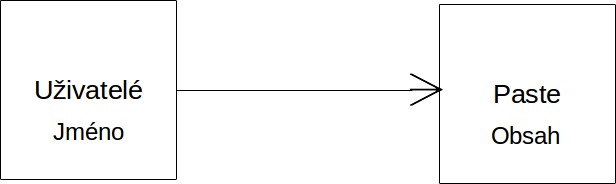
\includegraphics[scale=0.4]{dat_mod.png} 
  \caption{Datový model}
  \label{dat_mod}
\end{figure}

Relace mezi entitami slouží k vyjádření vztahu uživatelů a jejich pastů. Každý uživatel může mít bezpočet pastů. Na druhou stranu každý paste je jednoznačně přiřazen k uživateli.

\section{Uživatelské role}

Jak již bylo zmíněno výše, aplikace obsahuje dvě uživatelské role. Jednou z nich je anonymní role uživatele. Ta slouží pro náhodné vkladatele pastů. Oproti tomu existuje registrovaný uživatel, který je uchováván v databázi aplikace. 

\section{Návrh uživatelského rozhraní}

Uživatelské vychází z následujících Wireframů (ty jsou vytvořeny v aplikaci Pencil~\cite{pencil}):

\begin{figure}[H]
  \centering
	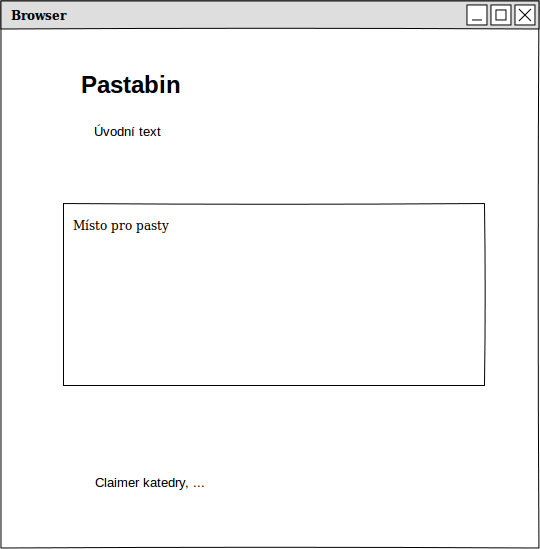
\includegraphics[scale=0.4]{uvod.png} 
  \caption{Úvodní obrazovka aplikace}
  \label{uvod_app}
\end{figure}

Wireframe obsahuje jen hrubý nárys aplikace. Není v něm zaneseno okénko pro přihlášení. Po vložení svého pastu se uživatel přenese do druhého okna aplikace. To už obsahuje samotný paste.

\begin{figure}[H]
  \centering
	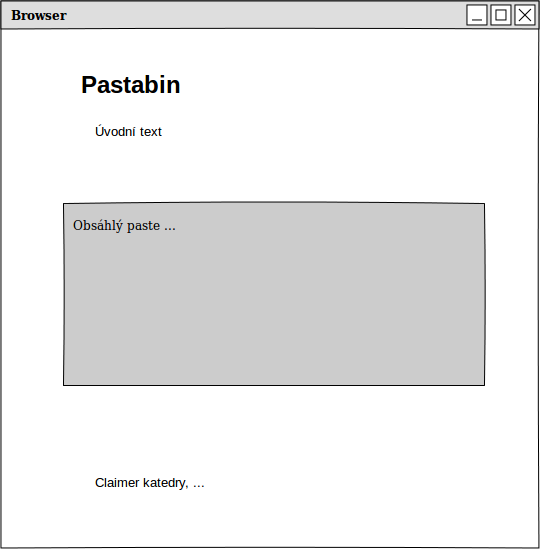
\includegraphics[scale=0.4]{pasty.png} 
  \caption{Úvodní obrazovka aplikace}
  \label{paste_app}
\end{figure}

\chapter{Technický specifikace}

V následující části textu jsou rozebrány technické prvky realizace portálu.

Pro vytvoření portálu na straně serveru byl použit jazyk \texttt{PHP}. S přihlédnutím ke kvalitnější metodice vývoje je použit framework \texttt{Nette}. Pomocí frameworku jsou vytvořeny nativní tři vrstvy aplikace (obrázek \ref{nette}). Nette používá relaxovaný model, takže je možné posloupnost vrstev porušit. V tomto projektu se tomu však nestalo.

\begin{figure}[H]
  \centering
	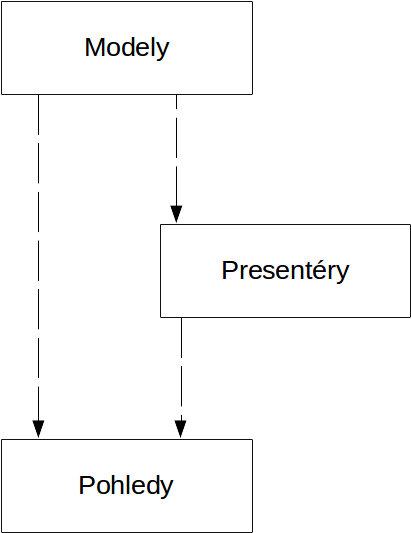
\includegraphics[scale=0.5]{nette.png} 
  \caption{Vrstvy frameworku \texttt{Nette}}
  \label{nette}
\end{figure}

Obsah vrstev je rozebrán v následujícím textu. V modelech jsou umístěny objekty mapující tabulky databáze. V prezentérech je připravován obsah pro uživatele, který je následně zobrazen pomocí pohledů. V jiné literatuře se můžeme setkat s pojmem kontrolér, \texttt{Nette} ale používá výraz prezentér \cite{nettfr}. 

\section{Relační model}

Pro uchování dat portálu byla použita databáze \texttt{MySQL}. \texttt{MySQL} používá vlastní návrhář entit, ten se jmenuje \texttt{MySQL WorkBench}. Pomocí tohoto nástroje je vytvořen digram \texttt{EER} zobrazující vztah mezi entitou uživatelů a jejich pasty.

\begin{figure}[H]
  \centering
	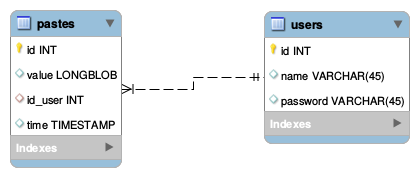
\includegraphics[scale=0.5]{EER.png} 
  \caption{\texttt{EER} reprezentace entit}
  \label{eer}
\end{figure}

Jak je vidět z digramu, vazba mezi uživateli a pasty je volná. Může existovat paste, který nikomu nepatří. Stejně tak může existovat uživatel, který nemá žádný paste.

Za zmínku stojí, že velikost pastů je omezena maximální velikostí datového typu \texttt{LONGBLOB}. Paste může být tedy doopravdy veliký. Při každém vložení paste je zaznamenán čas pomocí datové struktury \texttt{TIMESTAMP}. Čas zapisuje databáze pomocí následující \texttt{Default} hodnoty:

\begin{verbatim}
CURRENT_TIMESTAMP ON UPDATE CURRENT_TIMESTAMP
\end{verbatim}

Datový model je dále namapován na modely v architektuře aplikace. Ta je následující:

\begin{figure}[H]
  \centering
	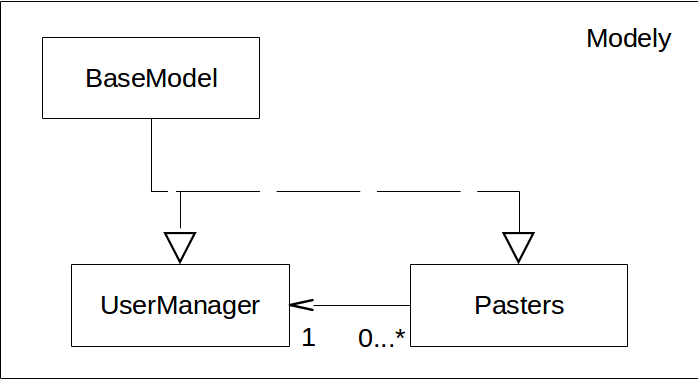
\includegraphics[scale=0.5]{modely.png} 
  \caption{Entity vrstvy modelů}
  \label{models}
\end{figure}

\texttt{BaseModel} je entita, která má za úkol vyvolat společné atributy následných tříd. Obsahuje tedy volání na databázi.

Za zmínku stojí třída \texttt{UserManager}, která spravuje třídy pro autentizaci, autorizaci a akounting. Všechny ostatní entity jsou už vestavěny ve frameworku \texttt{Nette}. Proto, ačkoliv nikde není reprezentace modelu uživatel, prezentéry pracují s entitou uživatel, která je volána právě z třídy \texttt{UserManager}.

Třída \texttt{Pasters} mapuje entitu \texttt{pastes} z datového modelu.

\section{Architektura aplikace}

Hlavní částí aplikace jsou prezéntéry. Ty mají za úkol připravit obsah portálu pro uživatele.

\begin{figure}[H]
  \centering
	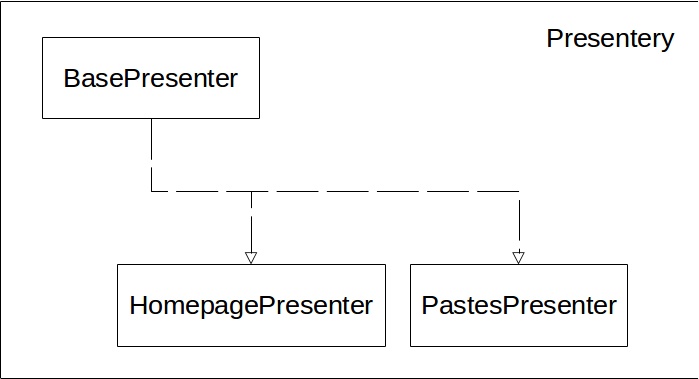
\includegraphics[scale=0.5]{presentery.png} 
  \caption{Entity vrstvy prezentérů}
  \label{presenter}
\end{figure}

Jak můžeme vidět, \texttt{BasePresenter} slouží zase jen k zavedení společných částí entit prezentační vrstvy.

\texttt{HomepagePresenter} slouží k reprezentaci funkcionality čelní stránky aplikace. Pokrývá většinu práce s uživatelem. Oproti tomu \texttt{PastesPresenter} pracuje už pouze s pasty na stránce.

\subsection{Pohledy}

Aplikace pracuje s pohledy, které jsou odvozeny z prezentérů. To znamená, že pro každý prezentér existuje aspoň jeden pohled. \texttt{Nette} pro vytváření pohledů používá jazyk \texttt{Latte}. Společné vlastnosti pohledů jsou v pohledu \texttt{@layout.latte}. V tom jsou rozvrženy pomocí bloků, které se mění podle toho, jak je prezentér nastaví.

V následující ukázce je vystižen celý layout stránky:

\begin{verbatim}
{**
 * @param string   $basePath web base path
 * @param array    $flashes  flash messages
 *}

<!DOCTYPE html>
<html>
<head>
	<meta charset="utf-8">

	<title>{ifset title}{include title|striptags} | {/ifset}Nette Sandbox</title>
	<link rel="stylesheet" href="{$basePath}/css/bootstrap.min.css">
	<link rel="stylesheet" href="{$basePath}/css/own.css">
	<link rel="shortcut icon" href="{$basePath}/favicon.ico">
	<meta name="viewport" content="width=device-width">
	{block head}{/block}
</head>

<body>

    <div class="container">
<div class="jumbotron">
	{ifset title_page}{include title_page}{/ifset}
</div>

	<div n:foreach="$flashes as $flash" n:class="flash, $flash->type">{$flash->message}</div>
	<div class="row marketing">
		{include content}
	</div>
 	<footer class="footer">
		<p>
Tato práce vznikla jako semestrální úloha z předmětu "Tvorba www aplikací".
		</p>
	</footer>
    </div>
	{block scripts}
	<script src="//code.jquery.com/jquery-1.11.3.min.js"></script>
	<script src="//nette.github.io/resources/js/netteForms.min.js"></script>
	<script src="{$basePath}/js/main.js"></script>
	<script src="{$basePath}/js/bootstrap.js"></script>
	<script src="{$basePath}/js/own.js"></script>
	{/block}
</body>
</html>
\end{verbatim}

Všimněte si vestavěného volání knihoven \texttt{JQuery} a použití základního stylování pomocí framework \texttt{Bootstrap}.

\chapter{Závěr}

Portál je koncepčně poměrně jednoduchý. Velkým problémem je zvolená metodika. Na jednu stranu je kvůli použití frameworků usnadněn následný rozvoj aplikace. Na druhou však je vývoj o to složitější, protože samotný framework není tak intuitivní, jak nativní \texttt{PHP}.

Pro hlubší pochopení portálu doporučují projít dokumentaci vygenerovanou pomocí \texttt{Doxygen}.

Celý projekt je na portálu \texttt{GitHub} \url{https://github.com/Nemo112/pastabin}.

\appendix

\chapter{Reference pojmů}

\begin{tabular}{| l | p{10cm} |}
\hline
Termín & popis \\
\hline
Paste & Vložený text pomocí \texttt{CTRL+C CTRL+V}. \\
Odkaz & V tomto textu chápáno podle standardu \texttt{URL}. \\
\texttt{EER} & Enhanced entity–relationship model. \\
Framework & Struktura pomáhající při vývoji aplikace. \\
\hline
\end{tabular}

\bibliography{mybib}
\bibliographystyle{csn690}

\end{document}
